\label{sec:empirical}
% Empirical	Approach
% Description of the empirical model: specification and variables involved
% Strategy for the estimation of the parameters of interest and test of the hypothesis
\subsection{Baseline model}
\label{subsec:e_model}
Our baseline model is a Random Effects (RE) model to be estimated using feasible Generalized Least Squares (fGLS). Electricity consumption $e$ for grid company $i$ at time $t$ (date by hour) is given by:
\begin{equation}
  \begin{split}
  \ln e_{it}=&\ \varepsilon \hat{\ln p_{rt}}+\delta\ln n_{im}+\bm{w}^{'}_{rt}\lambda+\gamma\ days\\
  &+\eta_{year}+\eta_{week}+\eta_{month}\cdot\eta_{hour}+\eta_{day}\cdot\eta_{hour}+\psi_i+u_{it}
  \end{split}
  \label{eq:baseline}
\end{equation}
Where $p$ is the electricity spot price in price region $r$ at time $t$, $n$ is the number of meters at the beginning of the month $m$, $\bm{w}$ is a vector of weather variables for the given price region $r$ at time $t$. Time variables include the time trend $days$. The $\eta$'s' represent dummies for each year and each ISO week number, as well as dummies for hour of the day interacted with each month and each day of the week respectively. $\psi_i$ is the grid-specific time-invariant constant term that is treated as random and $u_{it}$ is the idiosyncratic error term.
\par\vspace{-1em}
We use a log-log specification for electricity consumption, the spot price, and the number of meters as it allows us to model demand responses across grid areas of different size. Furthermore, log-log is the more standard specification which allows for a more direct comparison to the results in other studies \citep{burke2017price}. Other attractive properties include that the estimation provides the elasticity directly and does not predict non-positive electricity consumption, furthermore, the specification reduces the impact of outliers and are found to reduce systematic patterns in the estimated residuals \citep{burke2017price}.
\par\vspace{-1em}
The specification is first estimated for each hour of the days to identify peak-hours, off-peak, and the shoulder-period.

\subsection{Instrumenting for prices}
\label{subsec:e_instrumenting}
To circumvent the simultaneity problem described in section \ref{subsec:b_endogeneity} we consider using lagged prices or wind-power production as price instruments. This makes sense as the marginal cost of production is close to zero, such that a high expected wind-power production will increase the overall supply capacity and drive down the prices as seen in figure \ref{fig:wp_price_dk1_week} (and figure \ref{fig:wp_price_dk1_week} in appendix \ref{app:data} for DK2).
% As an over-production of wind power will lead to transmission to neighboring bidding areas, the wind-power production prognosis for the other bidding area in Denmark is also included as an instrument.
\begin{figure}[H]
  \centering
  \caption{Wind power prognosis and spot price by week (DK1)}
  \label{fig:wp_price_dk1_week}
    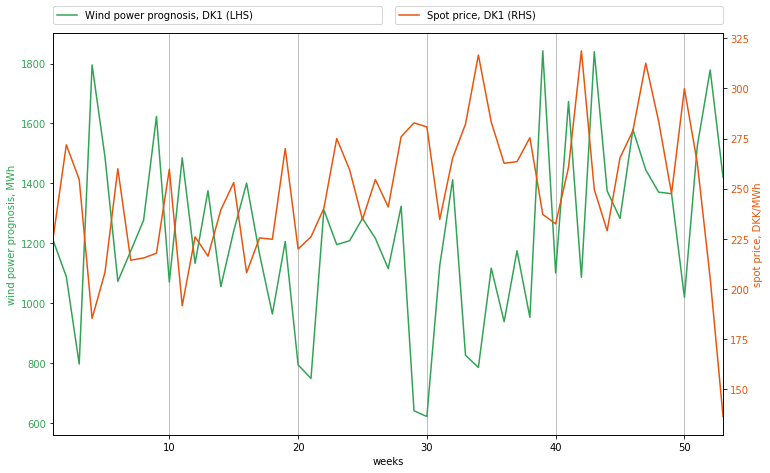
\includegraphics[width=1 \textwidth]{03_figures/wp_DK1_weeks}
\end{figure}

\subsection{Effect of Time-of-use tariff}
\label{subsec:e_tout}
Since 2018 flex-settled consumers in the Copenhagen metropolitan area are charged a time-of-use (TOU) tariff for the hours 17-19. To estimate this effect the baseline specification (\ref{eq:baseline}) is estimated for the hours 17-19 solely for the grid company Radius using 2SLS, thus, without the grid-area random effect $\psi_i$ but including a term for the effect of the TOU tariff:
\begin{align}
  \beta\frac{nf_{month}}{nr_{month}}\tau_{year,month}
  \label{eq:tout}
\end{align}
Where $nf$ is the number of flex-settled meters by month, $nr$ is the total number of meters for retail customers, and $\tau$ is a dummy for being in January-March or October-December in 2018. To isolate the effect of the TOU tariff we need to assume that residual consumers do not react on the tariff, on the contrary their consumption is assumed to follow the same hour-by-day, hour-by-month, and week patterns as the previous years and the effect of year dummies and the time trend to be evenly distributed across the year.\par\vspace{-1em}
As Figure \ref{fig:cons_meters_time_series} shows, a weakness is that the monthly records for the number of flex-settled meters provides a lack which can result in an upward bias of $\hat{\beta}$.


\subsection{Random Effects estimation}
\label{subsec:e_re}
Different candidates for panel data estimation
\begin{itemize}
    \item Least Squares Dummy Variables estimation (LSDV)
    \begin{itemize}
        \item Unobserved heterogeneity, $\psi_i>0$, leads to serial correlation
    \end{itemize}
    \item Fixed Difference estimation (FD)
    \begin{itemize}
        \item Strict exogeneity assumption, $cov(u_{it},\bm{x}_{it})=0$, is violated by hourly-patterns
    \end{itemize}
    \item Fixed Effects estimation (FE)
    \begin{itemize}
        \item Time-demeaned, too extreme
    \end{itemize}
    \item Dynamic Panel Estimation using Generalized Methods of Moments (GMM)
    \begin{itemize}
        \item Only necessary if including lagged prices as instruments
    \end{itemize}
\end{itemize}
We choose the \textbf{Random Effects estimator (RE)} for wholesale consumption
\begin{itemize}
    \item Critical assumption for RE: No endogeneity, i.e. $cov(\psi_i,\bm{x}_{it})=0$.
    \item Hausman test: $\hat{\beta_{RE}}=\hat{\beta_{FE}}$ no endogeneity, thus both RE and FE are consistent, but RE is more efficient.
\end{itemize}
Estimate RE estimation using \textbf{feasible Generalized Least Squares (fGLS)}
\begin{itemize}
    \item[\nth{1} stage:] Estimate eq. (\ref{eq:baseline}) using LSDV estimation $\rightarrow$ store $\hat{\lambda}=1-\left(\frac{\sigma^2_u}{\sigma^2_u+T\sigma^2_\alpha}\right)^\frac{1}{2}$
    \item[\nth{2} stage:] LSDV using $\hat{\lambda}$ to estimate the quasi-time demeaned system of the form: $y_{it}-\hat{\lambda}\bar{y_i}=\beta_0(1-\hat{\lambda})+\beta_1(\bm{x}_{it}-\hat{\lambda}\bar{\bm{x}_i})+\psi_i(1-\hat{\lambda})+u_{it}-\hat{\lambda}u_{it}$.
\end{itemize}

\subsection{Robustness checks}
\label{subsec:e_robustness}
The robustness of the elasticity for wholesale electricity demand in the peak-hours 12-15 is tested by splitting the sample by region, year, and month respectively to look for heterogeneous effects. Furthermore, we run do the estimation for each grid area and for the mean of each price region using 2SLS. As the FE estimates are identical, however less efficient, we also try to weight the estimates by the number of wholesale meters in each grid.
\medskip\\
Tests of the robustness of the effect of the TOU tariff is less straight forward. We try including the dummy constructed for Radius in estimation of retail electricity demand in different grids.
